\section{Resultados}


\subsection{Entrenando la última capa}

\subsubsection{ResNet-50}

\begin{figure}[H]
  \centering
  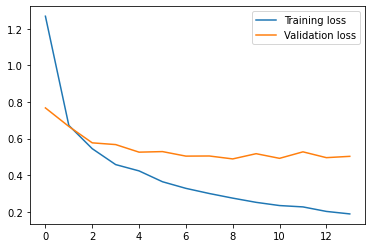
\includegraphics[width=0.5\linewidth]{Imagenes/entrenamiento_redes/ult/resnet_ult_loss.png}
  \caption{Perdida en ResNet50 entrenando unicamente la última capa.}
\end{figure}

\begin{figure}[H]
  \centering
  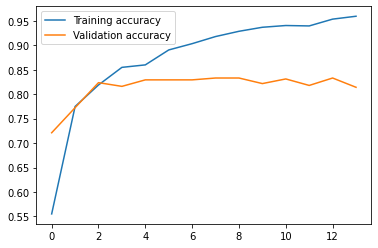
\includegraphics[width=0.5\linewidth]{Imagenes/entrenamiento_redes/ult/resnet_ult_acc.png}
  \caption{Precisión en ResNet50 entrenando unicamente la última capa.}
\end{figure}

\begin{figure}[H]
  \centering
  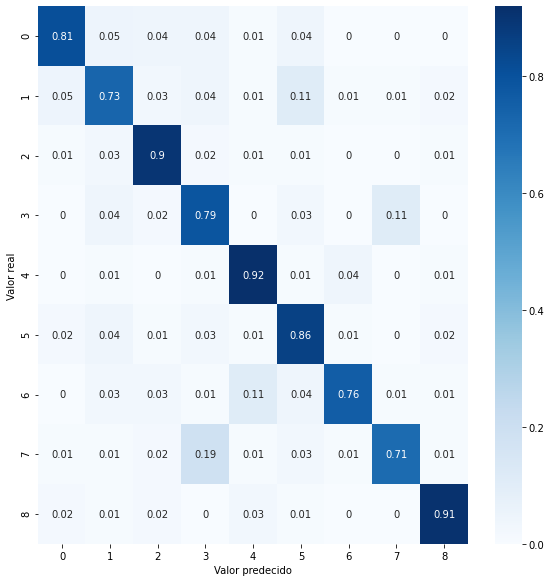
\includegraphics[width=0.5\linewidth]{Imagenes/entrenamiento_redes/ult/resnet_ult_matriz.png}
  \caption{Matriz de confusión sobre los datos de test en ResNet50 entrenando unicamente la última capa.}
\end{figure}

\begin{lstlisting}
Accuracy con ResNet50 entrenando solo ultima capa: 0.8180439727065959
\end{lstlisting}



\begin{figure}[H]
  \centering
  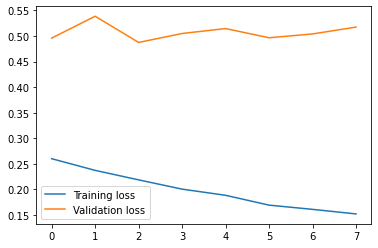
\includegraphics[width=0.5\linewidth]{Imagenes/entrenamiento_redes/ult/resnet_fine_loss.png}
  \caption{Perdida en ResNet50 entrenando unicamente la última capa y tras ajuste fino.}
\end{figure}

\begin{figure}[H]
  \centering
  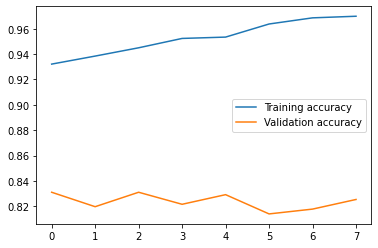
\includegraphics[width=0.5\linewidth]{Imagenes/entrenamiento_redes/ult/resnet_fine_acc.png}
  \caption{Precisión en ResNet50 entrenando unicamente la última capa y tras ajuste fino.}
\end{figure}

\begin{figure}[H]
  \centering
  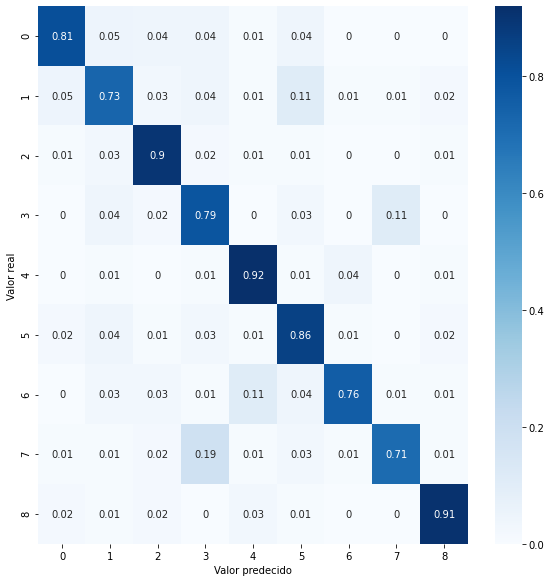
\includegraphics[width=0.5\linewidth]{Imagenes/entrenamiento_redes/ult/resnet_fine_matriz.png}
  \caption{Matriz de confusión sobre los datos de test en ResNet50 entrenando unicamente la última capa y tras ajuste fino..}
\end{figure}

\begin{lstlisting}
Accuracy con ResNet50 tras ajuste fino: 0.8180439727065959
\end{lstlisting}



\subsubsection{DenseNet-121}


\begin{figure}[H]
  \centering
  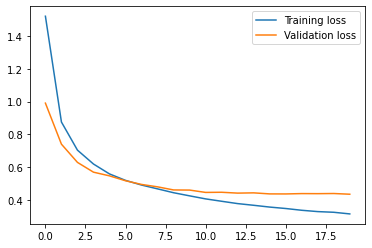
\includegraphics[width=0.5\linewidth]{Imagenes/entrenamiento_redes/ult/densenet_ult_loss.png}
  \caption{Perdida en DenseNet121 entrenando unicamente la última capa.}
\end{figure}

\begin{figure}[H]
  \centering
  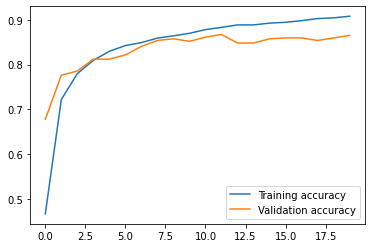
\includegraphics[width=0.5\linewidth]{Imagenes/entrenamiento_redes/ult/densenet_ult_acc.png}
  \caption{Precisión en DenseNet121 entrenando unicamente la última capa.}
\end{figure}

\begin{figure}[H]
  \centering
  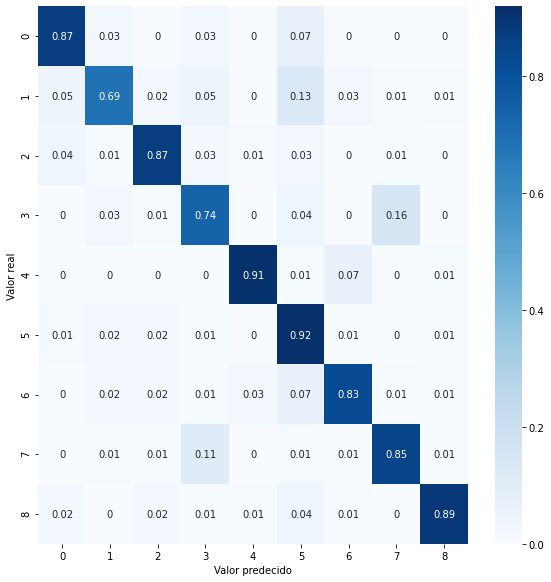
\includegraphics[width=0.5\linewidth]{Imagenes/entrenamiento_redes/ult/densenet_ult_matriz.png}
  \caption{Matriz de confusión sobre los datos de test en DenseNet121 entrenando unicamente la última capa.}
\end{figure}

\begin{lstlisting}
Accuracy con DenseNet121 entrenando solo ultima capa: 0.8377558756633814
\end{lstlisting}

Con DenseNet121, a diferencia que con ResNet50, vemos como no encontramos tanto sobreajuste tras las primeras épocas, aunque los valores de precisión en el conjunto de test son muy similares, aunque un poco mejores que en ResNet50. Observamos como de nuevo es capaz de clasificar las clases sin mucho problema, a excepción de un par de casos concretos que comentaremos al final de los resultados.



\begin{figure}[H]
  \centering
  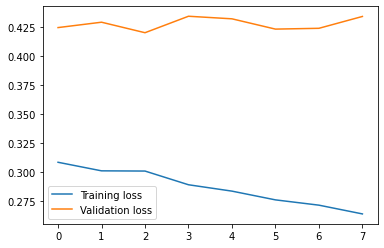
\includegraphics[width=0.5\linewidth]{Imagenes/entrenamiento_redes/ult/densenet_fine_loss.png}
  \caption{Perdida en DenseNet121 entrenando unicamente la última capa y tras ajuste fino.}
\end{figure}

\begin{figure}[H]
  \centering
  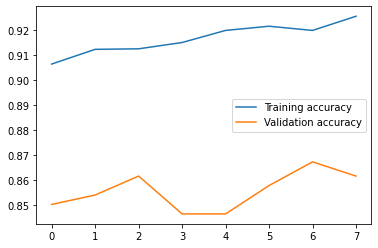
\includegraphics[width=0.5\linewidth]{Imagenes/entrenamiento_redes/ult/densenet_fine_acc.png}
  \caption{Precisión en DenseNet121 entrenando unicamente la última capa y tras ajuste fino.}
\end{figure}

\begin{figure}[H]
  \centering
  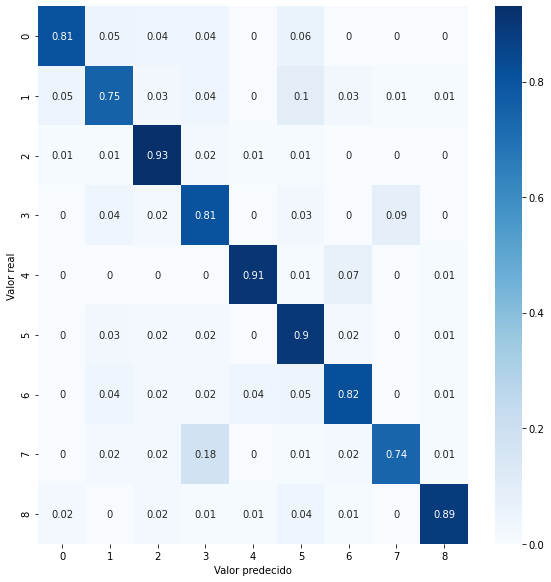
\includegraphics[width=0.5\linewidth]{Imagenes/entrenamiento_redes/ult/densenet_fine_matriz.png}
  \caption{Matriz de confusión sobre los datos de test en DenseNet121 entrenando unicamente la última capa y tras ajuste fino.}
\end{figure}


\begin{lstlisting}
Accuracy con DenseNet121 tras ajuste fino: 0.8385140257771039
\end{lstlisting}

Tras aplicar el fine tuning en DenseNet121 mejora muy levemente, de forma casi imperceptible. Como vemos, en ambos casos se ha obtenido buenos resultados lo que nos da a entender que en DenseNet121 los pesos de ImageNet funcionan bastante bien para nuestro problema.


\subsubsection{InceptionV3}

\begin{figure}[H]
  \centering
  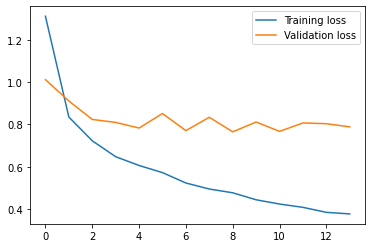
\includegraphics[width=0.5\linewidth]{Imagenes/entrenamiento_redes/ult/inception_ult_loss.png}
  \caption{Perdida en InceptionV3 entrenando unicamente la última capa.}
\end{figure}

\begin{figure}[H]
  \centering
  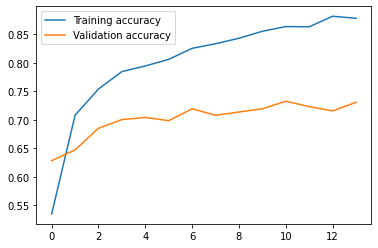
\includegraphics[width=0.5\linewidth]{Imagenes/entrenamiento_redes/ult/inception_ult_acc.png}
  \caption{Precisión en InceptionV3 entrenando unicamente la última capa.}
\end{figure}

\begin{figure}[H]
  \centering
  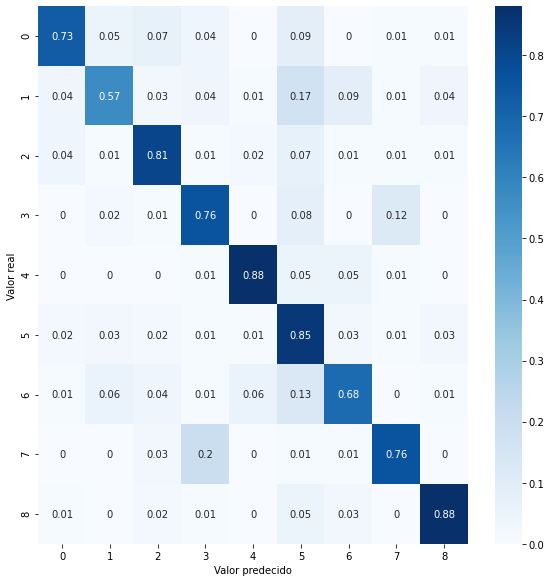
\includegraphics[width=0.5\linewidth]{Imagenes/entrenamiento_redes/ult/inception_ult_matriz.png}
  \caption{Matriz de confusión sobre los datos de test en InceptionV3 entrenando unicamente la última capa.}
\end{figure}


\begin{lstlisting}
Accuracy con InceptionV3 entrenando solo ultima capa: 0.7672479150871873
\end{lstlisting}


\begin{figure}[H]
  \centering
  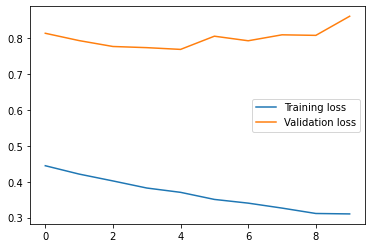
\includegraphics[width=0.5\linewidth]{Imagenes/entrenamiento_redes/ult/inception_fine_loss.png}
  \caption{Perdida en InceptionV3 entrenando unicamente la última capa y tras ajuste fino.}
\end{figure}

\begin{figure}[H]
  \centering
  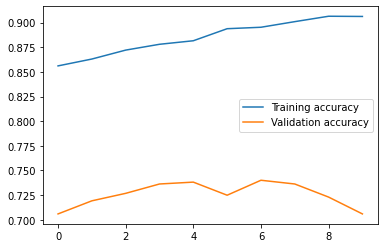
\includegraphics[width=0.5\linewidth]{Imagenes/entrenamiento_redes/ult/inception_fine_acc.png}
  \caption{Precisión en InceptionV3 entrenando unicamente la última capa y tras ajuste fino.}
\end{figure}

\begin{figure}[H]
  \centering
  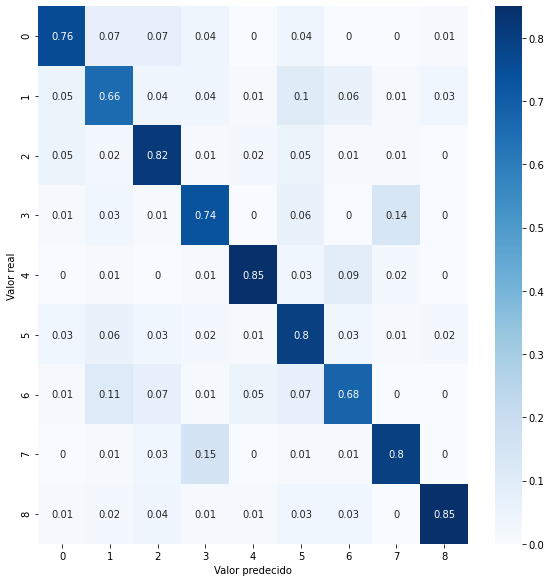
\includegraphics[width=0.5\linewidth]{Imagenes/entrenamiento_redes/ult/inception_fine_matriz.png}
  \caption{Matriz de confusión sobre los datos de test en InceptionV3 entrenando unicamente la última capa y tras ajuste fino.}
\end{figure}


\begin{lstlisting}
Accuracy con InceptionV3 tras ajuste fino: 0.7687642153146323
\end{lstlisting}


\subsubsection{EfficientNetB0}

\begin{figure}[H]
  \centering
  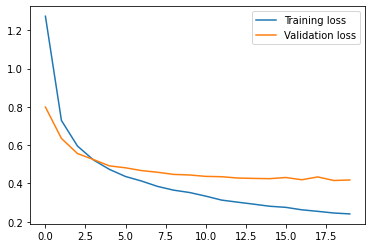
\includegraphics[width=0.5\linewidth]{Imagenes/entrenamiento_redes/ult/efficientnet_ult_loss.png}
  \caption{Perdida en EfficientNetB0 entrenando unicamente la última capa.}
\end{figure}

\begin{figure}[H]
  \centering
  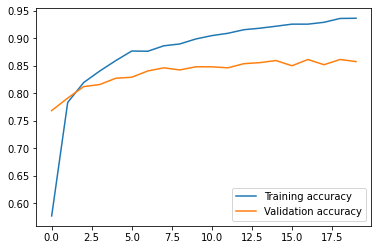
\includegraphics[width=0.5\linewidth]{Imagenes/entrenamiento_redes/ult/efficientnet_ult_acc.png}
  \caption{Precisión en EfficientNetB0 entrenando unicamente la última capa.}
\end{figure}

\begin{figure}[H]
  \centering
  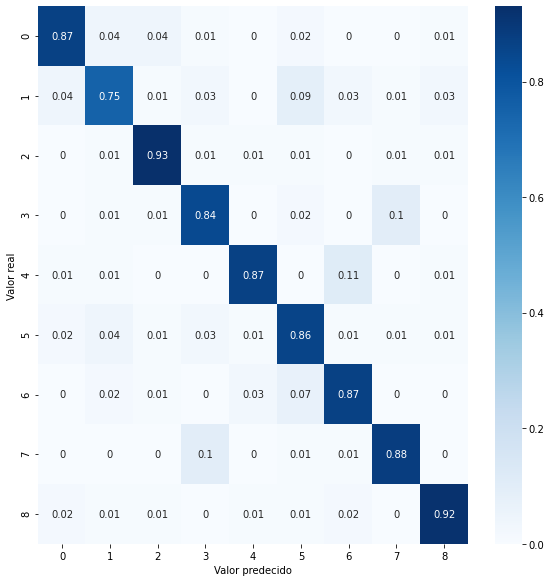
\includegraphics[width=0.5\linewidth]{Imagenes/entrenamiento_redes/ult/efficientnet_ult_matriz.png}
  \caption{Matriz de confusión sobre los datos de test en EfficientNetB0 entrenando unicamente la última capa.}
\end{figure}


\begin{lstlisting}
Accuracy con EfficientNetB0 entrenando solo ultima capa: 0.8612585291887794
\end{lstlisting}


\begin{figure}[H]
  \centering
  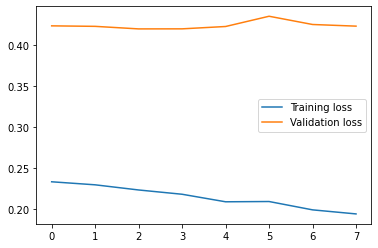
\includegraphics[width=0.5\linewidth]{Imagenes/entrenamiento_redes/ult/efficientnet_fine_loss.png}
  \caption{Perdida en EfficientNetB0 entrenando unicamente la última capa y tras ajuste fino.}
\end{figure}

\begin{figure}[H]
  \centering
  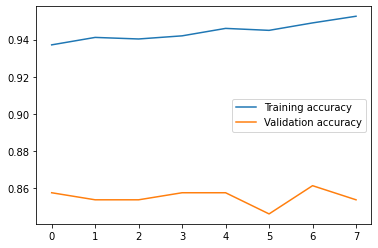
\includegraphics[width=0.5\linewidth]{Imagenes/entrenamiento_redes/ult/efficientnet_fine_acc.png}
  \caption{Precisión en EfficientNetB0 entrenando unicamente la última capa y tras ajuste fino.}
\end{figure}

\begin{figure}[H]
  \centering
  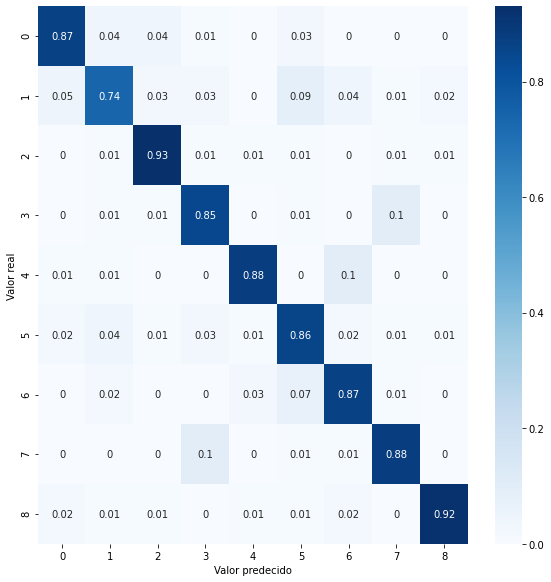
\includegraphics[width=0.5\linewidth]{Imagenes/entrenamiento_redes/ult/efficientnet_fine_matriz.png}
  \caption{Matriz de confusión sobre los datos de test en EfficientNetB0 entrenando unicamente la última capa y tras ajuste fino.}
\end{figure}

\begin{lstlisting}
Accuracy con EfficientNetB0 tras ajuste fino: 0.8627748294162244
\end{lstlisting}








% 5ult



\subsection{Entrenando las últimas cinco capas y añadiendo nuevas}

\subsubsection{ResNet-50}

\begin{figure}[H]
  \centering
  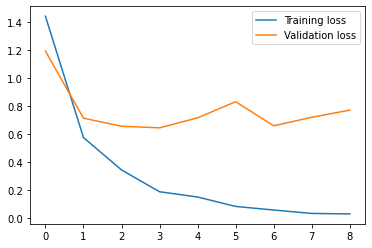
\includegraphics[width=0.5\linewidth]{Imagenes/entrenamiento_redes/5-ult/resnet_5ult_loss.png}
  \caption{Perdida en ResNet50 entrenando las cinco últimas capas y nuevas capas.}
\end{figure}

\begin{figure}[H]
  \centering
  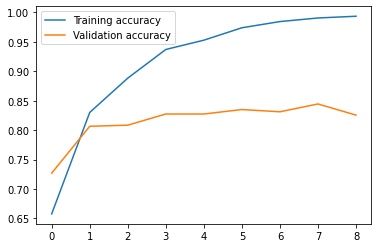
\includegraphics[width=0.5\linewidth]{Imagenes/entrenamiento_redes/5-ult/resnet_5ult_acc.png}
  \caption{Precisión en ResNet50 entrenando las cinco últimas capas y nuevas capas.}
\end{figure}

\begin{figure}[H]
  \centering
  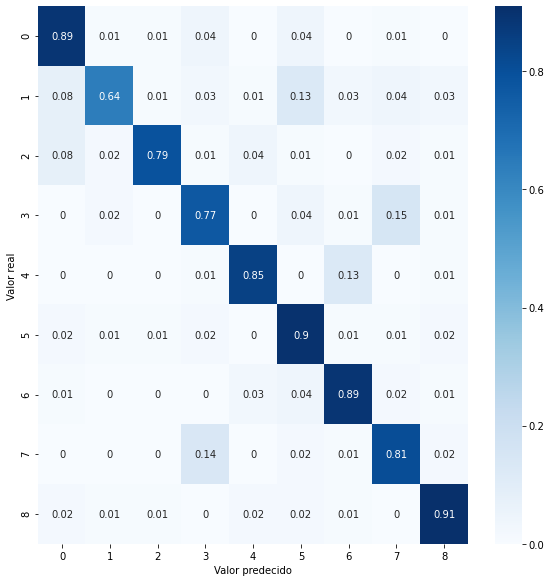
\includegraphics[width=0.5\linewidth]{Imagenes/entrenamiento_redes/5-ult/resnet_5ult_matriz.png}
  \caption{Matriz de confusión sobre los datos de test en ResNet50 entrenando las cinco últimas capas y nuevas capas.}
\end{figure}

\begin{lstlisting}
Accuracy con ResNet50 entrenando las cinco últimas capas: 0.821076573161486
\end{lstlisting}




\begin{figure}[H]
  \centering
  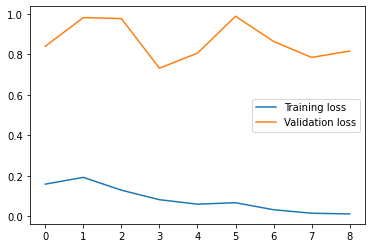
\includegraphics[width=0.5\linewidth]{Imagenes/entrenamiento_redes/5-ult/resnet_5fine_loss.png}
  \caption{Perdida en ResNet50 entrenando las cinco últimas capas y nuevas capas tras ajuste fino.}
\end{figure}

\begin{figure}[H]
  \centering
  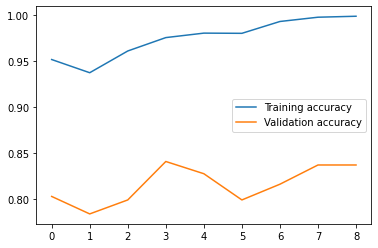
\includegraphics[width=0.5\linewidth]{Imagenes/entrenamiento_redes/5-ult/resnet_5fine_acc.png}
  \caption{Precisión en ResNet50 entrenando las cinco últimas capas y nuevas capas tras ajuste fino.}
\end{figure}

\begin{figure}[H]
  \centering
  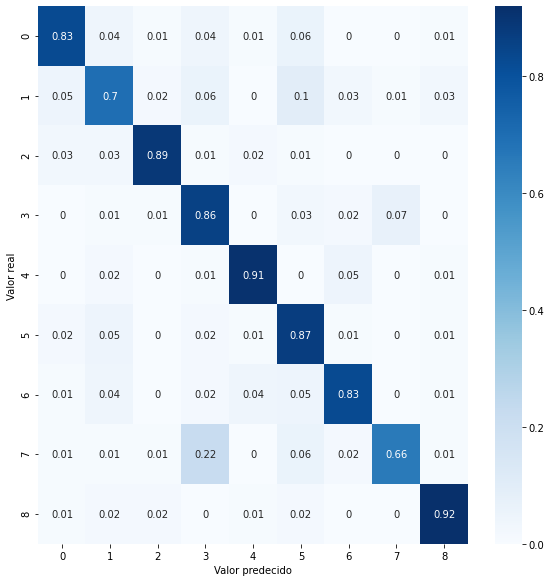
\includegraphics[width=0.5\linewidth]{Imagenes/entrenamiento_redes/5-ult/resnet_5fine_matriz.png}
  \caption{Matriz de confusión sobre los datos de test en ResNet50 entrenando las cinco últimas capas y nuevas capas tras ajuste fino..}
\end{figure}


\begin{lstlisting}
Accuracy con ResNet50 tras ajuste fino: 0.8256254738438211
\end{lstlisting}


\subsubsection{DenseNet-121}

\begin{figure}[H]
  \centering
  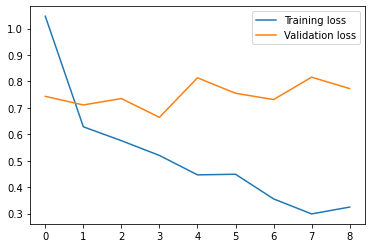
\includegraphics[width=0.5\linewidth]{Imagenes/entrenamiento_redes/5-ult/densenet_5ult_loss.png}
  \caption{Perdida en DenseNet121 entrenando las cinco últimas capas y nuevas capas.}
\end{figure}

\begin{figure}[H]
  \centering
  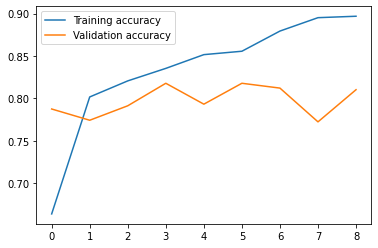
\includegraphics[width=0.5\linewidth]{Imagenes/entrenamiento_redes/5-ult/densenet_5ult_acc.png}
  \caption{Precisión en DenseNet121 entrenando las cinco últimas capas y nuevas capas.}
\end{figure}

\begin{figure}[H]
  \centering
  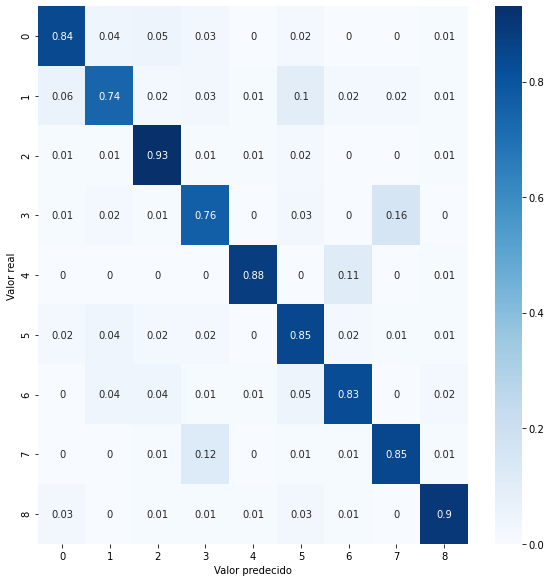
\includegraphics[width=0.5\linewidth]{Imagenes/entrenamiento_redes/5-ult/densenet_5ult_matriz.png}
  \caption{Matriz de confusión sobre los datos de test en DenseNet121 entrenando las cinco últimas capas y nuevas capas.}
\end{figure}


\begin{lstlisting}
Accuracy con DenseNet121 entrenando las ultimas 5 capas: 0.8339651250947687
\end{lstlisting}



\begin{figure}[H]
  \centering
  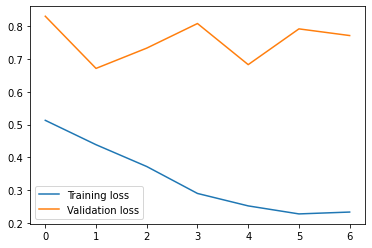
\includegraphics[width=0.5\linewidth]{Imagenes/entrenamiento_redes/5-ult/densenet_5fine_loss.png}
  \caption{Perdida en DenseNet121 entrenando las cinco últimas capas y nuevas capas tras ajuste fino.}
\end{figure}

\begin{figure}[H]
  \centering
  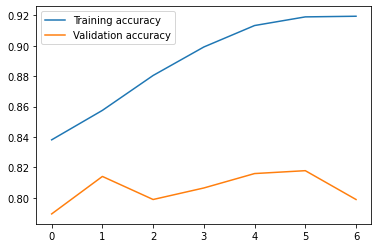
\includegraphics[width=0.5\linewidth]{Imagenes/entrenamiento_redes/5-ult/densenet_5fine_acc.png}
  \caption{Precisión en DenseNet121 entrenando las cinco últimas capas y nuevas capas tras ajuste fino.}
\end{figure}

\begin{figure}[H]
  \centering
  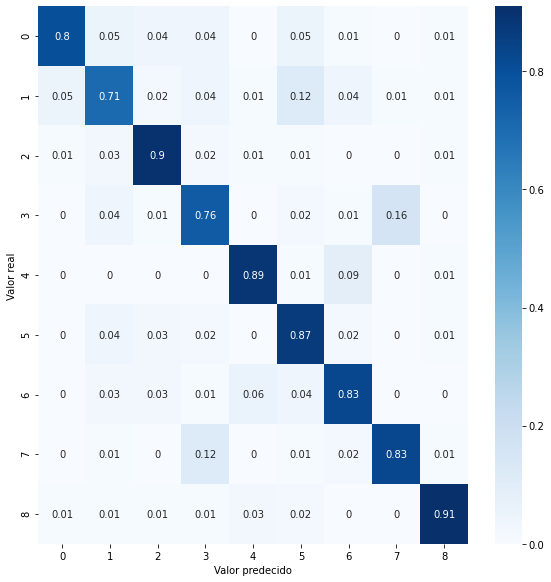
\includegraphics[width=0.5\linewidth]{Imagenes/entrenamiento_redes/5-ult/densenet_5fine_matriz.png}
  \caption{Matriz de confusión sobre los datos de test en DenseNet121 entrenando las cinco últimas capas y nuevas capas tras ajuste fino.}
\end{figure}

\begin{lstlisting}
Accuracy con DenseNet121 tras ajuste fino: 0.8263836239575436
\end{lstlisting}



\subsubsection{InceptionV3}


\begin{figure}[H]
  \centering
  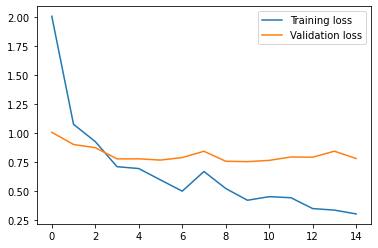
\includegraphics[width=0.5\linewidth]{Imagenes/entrenamiento_redes/5-ult/inception_5ult_loss.png}
  \caption{Perdida en InceptionV3 entrenando las cinco últimas capas y nuevas capas.}
\end{figure}

\begin{figure}[H]
  \centering
  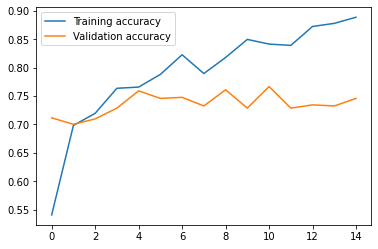
\includegraphics[width=0.5\linewidth]{Imagenes/entrenamiento_redes/5-ult/inception_5ult_acc.png}
  \caption{Precisión en InceptionV3 entrenando las cinco últimas capas y nuevas capas.}
\end{figure}

\begin{figure}[H]
  \centering
  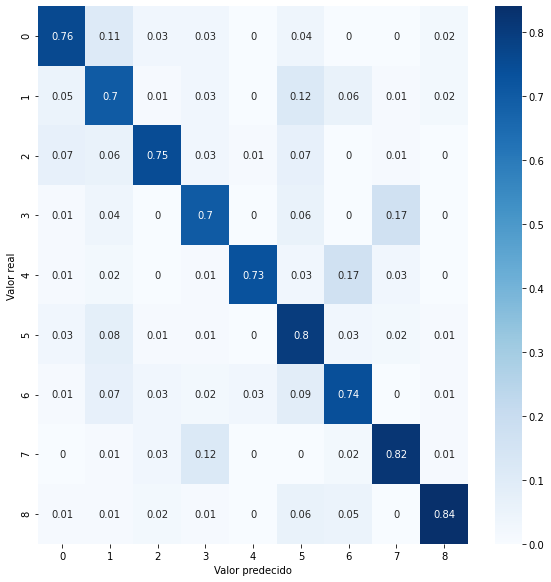
\includegraphics[width=0.5\linewidth]{Imagenes/entrenamiento_redes/5-ult/inception_5ult_matriz.png}
  \caption{Matriz de confusión sobre los datos de test en InceptionV3 entrenando las cinco últimas capas y nuevas capas.}
\end{figure}


\begin{lstlisting}
Accuracy con InceptionV3 entrenando las cinco últimas capas: 0.7589082638362395
\end{lstlisting}


\begin{figure}[H]
  \centering
  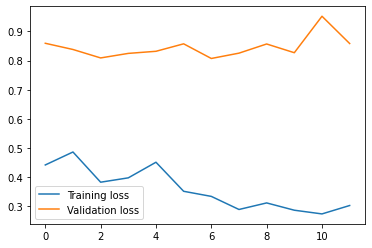
\includegraphics[width=0.5\linewidth]{Imagenes/entrenamiento_redes/5-ult/inception_5fine_loss.png}
  \caption{Perdida en InceptionV3 entrenando las cinco últimas capas y nuevas capas tras ajuste fino.}
\end{figure}

\begin{figure}[H]
  \centering
  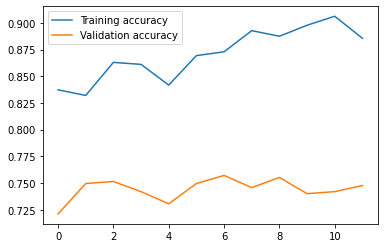
\includegraphics[width=0.5\linewidth]{Imagenes/entrenamiento_redes/5-ult/inception_5fine_acc.png}
  \caption{Precisión en InceptionV3 entrenando las cinco últimas capas y nuevas capas tras ajuste fino.}
\end{figure}

\begin{figure}[H]
  \centering
  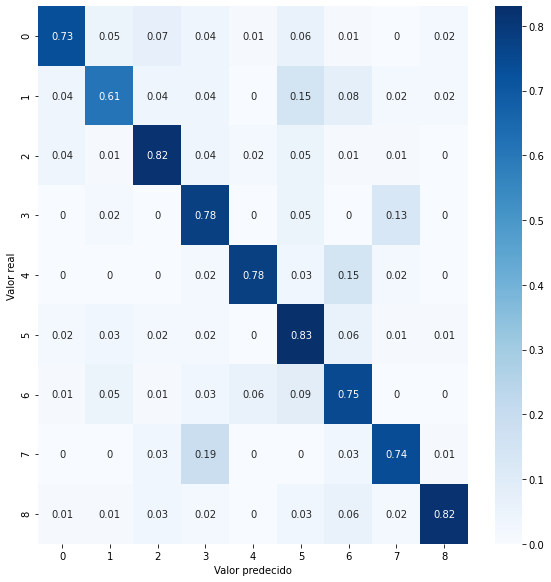
\includegraphics[width=0.5\linewidth]{Imagenes/entrenamiento_redes/5-ult/inception_5fine_matriz.png}
  \caption{Matriz de confusión sobre los datos de test en InceptionV3 entrenando las cinco últimas capas y nuevas capas tras ajuste fino.}
\end{figure}


\begin{lstlisting}
Accuracy con InceptionV3 tras ajuste fino: 0.7649734647460197
\end{lstlisting}



\subsubsection{EfficientNetB0}


\begin{figure}[H]
  \centering
  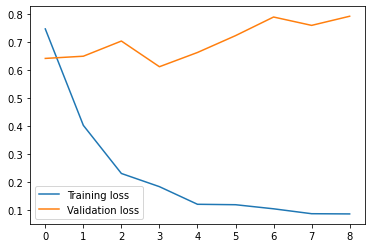
\includegraphics[width=0.5\linewidth]{Imagenes/entrenamiento_redes/5-ult/efficientnet_5ult_loss.png}
  \caption{Perdida en EfficientNetB0 entrenando las cinco últimas capas y nuevas capas.}
\end{figure}

\begin{figure}[H]
  \centering
  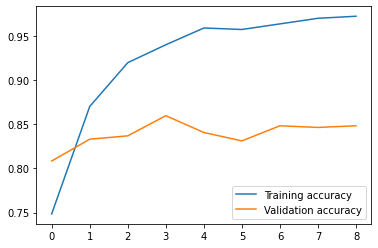
\includegraphics[width=0.5\linewidth]{Imagenes/entrenamiento_redes/5-ult/efficientnet_5ult_acc.png}
  \caption{Precisión en EfficientNetB0 entrenando las cinco últimas capas y nuevas capas.}
\end{figure}

\begin{figure}[H]
  \centering
  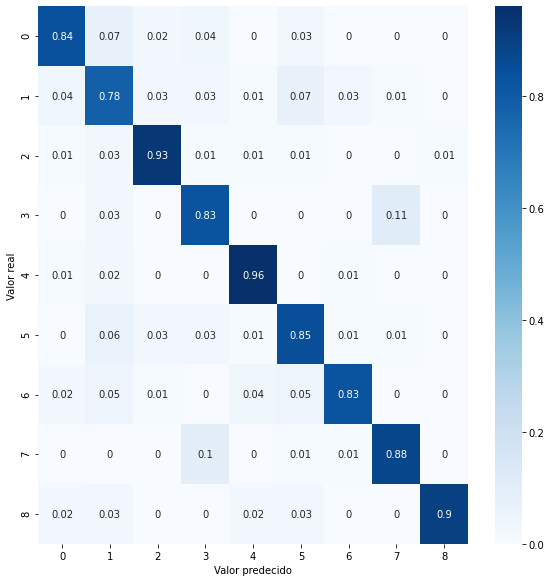
\includegraphics[width=0.5\linewidth]{Imagenes/entrenamiento_redes/5-ult/efficientnet_5ult_matriz.png}
  \caption{Matriz de confusión sobre los datos de test en EfficientNetB0 entrenando las cinco últimas capas y nuevas capas.}
\end{figure}


\begin{lstlisting}
Accuracy con EfficientNetB0 entrenando las cinco últimas capas: 0.8597422289613343
\end{lstlisting}


\begin{figure}[H]
  \centering
  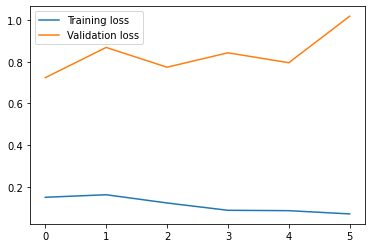
\includegraphics[width=0.5\linewidth]{Imagenes/entrenamiento_redes/5-ult/efficientnet_5fine_loss.png}
  \caption{Perdida en EfficientNetB0 entrenando las cinco últimas capas y nuevas capas tras ajuste fino.}
\end{figure}

\begin{figure}[H]
  \centering
  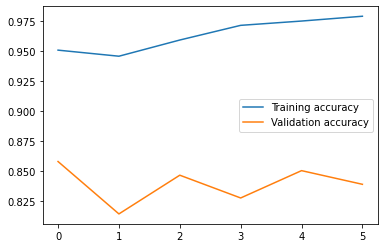
\includegraphics[width=0.5\linewidth]{Imagenes/entrenamiento_redes/5-ult/efficientnet_5fine_acc.png}
  \caption{Precisión en EfficientNetB0 entrenando las cinco últimas capas y nuevas capas tras ajuste fino.}
\end{figure}

\begin{figure}[H]
  \centering
  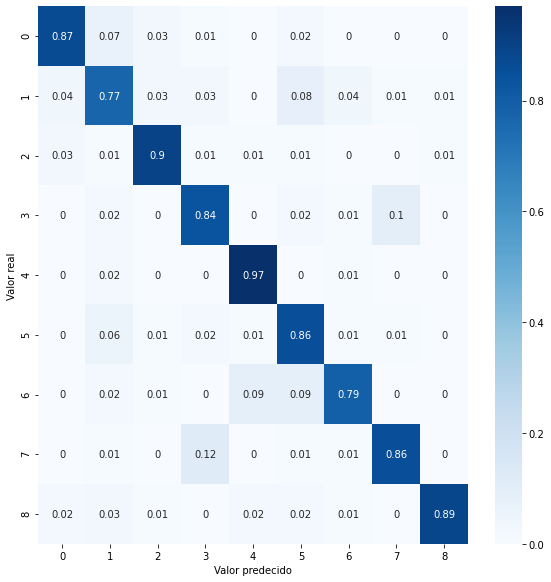
\includegraphics[width=0.5\linewidth]{Imagenes/entrenamiento_redes/5-ult/efficientnet_5fine_matriz.png}
  \caption{Matriz de confusión sobre los datos de test en EfficientNetB0 entrenando las cinco últimas capas y nuevas capas tras ajuste fino.}
\end{figure}


\begin{lstlisting}
Accuracy con EfficientNetB0 tras ajuste fino: 0.8567096285064443
\end{lstlisting}
